\documentclass[a4paper,11pt]{article}
\usepackage[T1]{fontenc}      % codifica dei font
\usepackage[utf8]{inputenc}
\usepackage[italian]{babel}
\usepackage{lipsum}
\usepackage{url}
\usepackage{amsfonts}
\usepackage{graphicx}
\begin{document}
% lettere accentate da tastiera
% lingua del documento
% genera testo fittizio
% per scrivere gli indirizzi Internet
\author{Linpeng Zhang}
\title{Tutorato AFL}
\maketitle
\begin{abstract}
    Per errori/dubbi/problemi: linpeng.zhang@studenti.unipd.it.% \\Note: 
\end{abstract}
\tableofcontents
\section{Lez4}
\subsection{Riassunto informale}
\begin{itemize}
    \item le grammatiche libere dal contesto accettano tutti i linguaggi regolari e qualcosa in più: infatti a lezione avete visto linguaggi non regolari (dimostrabile con il PL) che però potevano essere accettati da qualche CFG;
    \item in genere, data una CFG G, per dimostrare che $L=L(G)$ si dimostra sia che $L\subseteq L(G) \:$ e $L\supseteq L(G)$; spesso la prima parte si fa per induzione sulla lunghezza della stringa, mentre la seconda per induzione sul numero di passi di derivazione;
\end{itemize}
%Un automa a stati finiti, come suggerisce il nome, ha una "memoria limitata". Il mio consiglio per definire un automa che accetti un determinato linguaggio è pensare a cosa rappresenti ciascuno stato. Si noti infine che per essere sicuri che un automa riconosca un certo linguaggio bisognerebbe dimostrarlo (altrimenti non saremo mai sicuri). Ad esempio si possono dimostrare delle proprietà degli stati, o per induzione. Tuttavia, in genere, ciò non è richiesto.
\subsection{Esercizi}
\subsubsection{Esercizio 1}
Minimizzare il seguente automa.
\begin{minipage}{\linewidth}
    \centering
    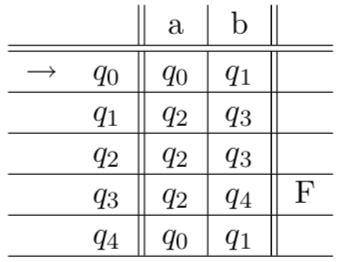
\includegraphics[width=5cm]{Lez4min.png}
\end{minipage}
\subsubsection{Esercizio 2}
Definire il linguaggio che accetta la CFG: $S\rightarrow aS|Sb|a|b$ e dimostrare la propria asserzione.
   \subsubsection{Esercizio 3}
    Siano dati una serie di linguaggi:
    \begin{enumerate}
        \item $L=\{0^m1^n,m\leq n,$ $n,m\in \mathbb{N}\}$
        \item $L=\{0^m1^n,n\neq m,$ $n,m\in \mathbb{N}\}$
        \item $L=\{x\in\{a,b\}^{*}|$ il numero di a è minore del numero di b $\}$
    \end{enumerate}
    Dire per ognuno di essi se:
    \begin{itemize}
        \item il linguaggio è regolare? Motivare la risposta;
        \item fornire, se esiste, una CFG che genera L e mostrarne la correttezza;
    \end{itemize}

    \subsection{Soluzioni}
    \subsubsection{Esercizio 1}
    \begin{minipage}{\linewidth}
        \centering
        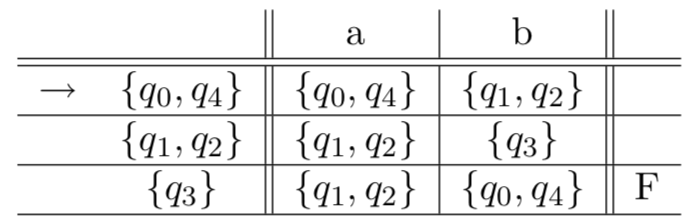
\includegraphics[width=5cm]{Lez4minsol.png}
    \end{minipage}
    \subsubsection{Esercizio 2}
Si ha $L(G)=\{a^nb^m|n,m\in\mathbb{N},n+m\geq 1\}=L$. L'asserzione va dimostrata per induzione in entrambi i versi. Una traccia alla dimostrazione è la seguente:
\begin{enumerate}
    \item ("$\Rightarrow$")\\Caso base: 1 derivazione, cioè $S\Rightarrow a$ o $S\Rightarrow b$ entrambe apparteSnenti a $L$.\\Caso induttivo: $S\Rightarrow aS\Rightarrow ^{n}aw'$ o $S\Rightarrow bS\Rightarrow ^{n}bw'$, ma $w' \in L$ per ipotesi induttiva. Aggiungendo una $a$ all'inizio o una $b$ alla fine rimane comunque una stringa in $L$;
    \item ("$\Leftarrow$")\\Caso base: lunghezza 1, cioè $w=a$ o $w=b$. Naturalmente $L(G)$ contiene queste stringhe perché ci sono direttamente le produzioni che lo fanno.\\Caso induttivo: $|w|=n+1$. Allora $w=w'b$ o $w=aw'$. Per ipotesi induttiva $S=>^{*}w'$. Quindi: $S\Rightarrow aS\Rightarrow aw'=w$ o $S\Rightarrow bS\Rightarrow bw'=w \: \Rightarrow w\in L(G)$.
\end{enumerate}
\subsubsection{Esercizio 3}
Le asserzioni che seguono vanno dimostrate.
    \begin{enumerate}
        %CFG 4,
        \item si può dimostrare con il PL che $L$ non è regolare. Una possibile CFG è: $S \rightarrow \epsilon | 0S1 | S1$;
        \item si può dimostrare con il PL che $L$ non è regolare, utilizzando ad esempio $w=0^h1^{h+h!} \: y=0^m$ e "pompando" con $k=1+h!/m$ (questi valori sono stati trovati utilizzando un k generico quando si va a "pompare" e imponendo di avere lo stesso numeri di 0 e di 1; il fattoriale garantisce che k sia intero). Notiamo che una parola o ha più zeri o ha più uni. Possiamo allora sfruttare la CFG precedente per scrivere la seguente:\\
        \begin{minipage}{\linewidth}
            \centering $S \rightarrow A | B$\\
            \centering $A \rightarrow \epsilon | 0A1 | A1$\\
            \centering $B \rightarrow \epsilon | 0B1 | 0B$\\
        \end{minipage}
        \item si può dimostrare con il PL che $L$ non è regolare. Intuitivamente per trovare una CFG notiamo che data una stringa in $L_2$ che ha $n_b$ occorrenze di b e $n_a$ occorrenze di a, allora o $n_b=n_a+1$ o $n_b>n_a+1$. In particolare:
        \begin{enumerate}
            \item nel primo caso, le stringhe saranno del tipo $ebe$ dove e è una stringa con $n_a=n_b$;
            \item nel secondo caso, le stringhe saranno costituite dalla concatenazione di due stringhe entrambe appartenenti a $L$;
        \end{enumerate}
        segue allora la seguente CFG:\\
        \begin{minipage}{\linewidth}
            \centering provate voi, la soluzione sarà presentata la prossima settimana.%$S \rightarrow EbE | SS$\\
            %\centering $E \rightarrow \epsilon | aEb | bEa | EE$
        \end{minipage}
  \end{enumerate}
    % Bibliografia
    %\begin{thebibliography}{9}
        %  Alcune soluzio
    %\end{thebibliography}
    \end{document}